%%% Please replace what is within each curly bracket with the correct information below. %%%
%%% The first field is already filled in for you.  %%%

\def\ClassName {15281} % Your course 


%\solution{
% \fbox{\begin{minipage}[t][5cm][t]{13cm} \Answer \end{minipage}} 
% }
%%%%% FILL IN YOUR ANSWERS TO EACH QUESTION BY REPLACE WHAT IS IN THE CURLY BRACKETS.
\def\Answer{\textbf{Put your answer here:}}
\def\AnswerNoPrompt{}

%%COMMENT OUT TO PRODUCE BLANK DOCUMENT
\def \showSolutions{}

\documentclass[twoside]{article}
\usepackage{placeins}
\usepackage{class}
\usepackage{graphicx}
\graphicspath{{./figs/}}
\usepackage{amsmath, amsthm, amssymb}
\usepackage{url} 
\usepackage{enumerate}
\usepackage{wrapfig}
\usepackage{enumitem}
\usepackage{color}
\usepackage{pifont}
\usepackage{mdwlist}
\usepackage[lofdepth,lotdepth]{subfig}
\usepackage{mdwlist}
\usepackage[ampersand]{easylist}
\usepackage{wasysym}
\usepackage{tikz}

\usetikzlibrary{shapes.geometric}
\usetikzlibrary{positioning}

\ListProperties(Hide=100, Hang=true, Progressive=3ex, Style*=-- ,
Style2*=$\bullet$ ,Style3*=$\circ$ ,Style4*=\tiny$\blacksquare$ )
\title{HW2}
\usepackage{multirow}

\pagestyle{myheadings}

\renewcommand{\P}{\mathbf{P}}
\newcommand{\eat}[1]{\ignorespaces}
\newcommand{\todo}[1]{ {\color{blue} TODO: #1} }
\newcommand{\X}{\ding{110}}
\newcommand{\F}{$\bullet$}
\newcommand{\Pac}{$<$}
\newcommand{\bigCI}{\mathrel{\text{\scalebox{1.07}{$\perp\mkern-10mu\perp$}}}}
\def\truefalse{\vspace{0.3in} \item (\emph{true} or \emph{false}) }
\def\indep{\perp\!\!\!\perp}
\def\sgn{\mathop{\mathrm{sign}}}
\newcommand{\solutionspace}[4]{\fbox{\begin{minipage}[t][#1][t]{#2} \textbf{#3} 

\solution{}{#4} \end{minipage}}}

% Bubbles for multiple choice questions
\newcommand{\emptycircle}{$\Large\bigcirc$}
\newcommand{\filledcircle}{$\Large\newmoon$}
\newcommand{\mcqb}{$\bigcirc$\ \ }
\newcommand{\mcqs}{\solution{\mcqb}{$\Large\newmoon$\ \ }}
\newcommand{\emptysquare}{{\Large $\square$}\ \ }
\newcommand{\filledsquare}{{\Large $\boxtimes$}\ \ }
\newcommand{\squaresolution}{\solution{\emptysquare}{\filledsquare}}


\begin{document}
\thispagestyle{empty}

\def\Name {Ishraaq Shams}  % Your name
\def\AndrewID{ishams} % Your andrewID
\def\Hours{} % The number of hours spent on this assignment


%%%%%%%%%%%%%%%%%%%%%%%%%%%%%%%%%%%%%%%%%%%%%%%%%%%
%%%%%%%%%%%%%%%%%%%% Problem 1 %%%%%%%%%%%%%%%%%%%%
%%%%%%%%%%%%%%%%%%%%%%%%%%%%%%%%%%%%%%%%%%%%%%%%%%%
\def \Onea{}
\def \Oneb{}
\def \Onecmax{}
\def \Onecmaxexample{}
\def \OnedYes{ 
    \emptycircle
    % \filledcircle
}
\def \OnedNo{
    \emptycircle
    % \filledcircle
}
\def \Onedreason{}
\def \OneeYes{
    \emptycircle
    % \filledcircle
}
\def \OneeNo{
    \emptycircle
    % \filledcircle
}
\def \Oneereason{}
\def \OnefYes{
    \emptycircle
    % \filledcircle
}
\def \OnefNo{
    \emptycircle
    % \filledcircle
}
\def \OnegYes{
    \emptycircle
    % \filledcircle
}
\def \OnegNo{
    \emptycircle
    % \filledcircle
}
\def \Oneh{}

%%%%%%%%%%%%%%%%%%%%%%%%%%%%%%%%%%%%%%%%%%%%%%%%%%%
%%%%%%%%%%%%%%%%%%%% Problem 2 %%%%%%%%%%%%%%%%%%%%
%%%%%%%%%%%%%%%%%%%%%%%%%%%%%%%%%%%%%%%%%%%%%%%%%%%
\def \Twoa{}
\def \Twob{}
\def \Twoc{}

%%%%%%%%%%%%%%%%%%%%%%%%%%%%%%%%%%%%%%%%%%%%%%%%%%%
%%%%%%%%%%%%%%%%%%%% Problem 3 %%%%%%%%%%%%%%%%%%%%
%%%%%%%%%%%%%%%%%%%%%%%%%%%%%%%%%%%%%%%%%%%%%%%%%%%
\def \Threeai{}
\def \Threeaii{}
\def \Threeaiii{}
\def \Threeaiv{}
\def \Threeav{}
\def \Threeavi{}
\def \Threeavii{}
\def \Threeaviii{}
\def \Threeaix{}
\def \Threeax{}
\def \Threeaxi{}
\def \Threeaxii{}
\def \Threeaxiii{}
\def \Threeaxiv{}
\def \Threeaxv{}
\def \Threeb{}
\def \ThreeCAdmissibleYes {
    \emptycircle
    % \filledcircle
}
\def \ThreeCAdmissibleNo {
    \emptycircle
    % \filledcircle
}
\def \ThreeCConsistentYes {
    \emptycircle
    % \filledcircle
}
\def \ThreeCConsistentNo {
    \emptycircle
    % \filledcircle
}
\def \ThreeDAdmissibleYes {
    \emptycircle
    % \filledcircle
}
\def \ThreeDAdmissibleNo {
    \emptycircle
    % \filledcircle
}
\def \ThreeDConsistentYes {
    \emptycircle
    % \filledcircle
}
\def \ThreeDConsistentNo {
    \emptycircle
    % \filledcircle
}


%%%%%%%%%%%%%%%%%%%%%%%%%%%%%%%%%%%%%%%%%%%%%%%%%%%
%%%%%%%%%%%%%%%%%%%% Problem 4 %%%%%%%%%%%%%%%%%%%%
%%%%%%%%%%%%%%%%%%%%%%%%%%%%%%%%%%%%%%%%%%%%%%%%%%%
\def \FourAATrue {
    \emptycircle
    % \filledcircle
}
\def \FourAAFalse {
    \emptycircle
    % \filledcircle
}
\def \FourABTrue {
    \emptycircle
    % \filledcircle
}
\def \FourABFalse {
    \emptycircle
    % \filledcircle
}
\def \FourACTrue {
    \emptycircle
    % \filledcircle
}
\def \FourACFalse {
    \emptycircle
    % \filledcircle
}
\def \FourADTrue {
    \emptycircle
    % \filledcircle
}
\def \FourADFalse {
    \emptycircle
    % \filledcircle
}
\def \FourAETrue {
    \emptycircle
    % \filledcircle
}
\def \FourAEFalse {
    \emptycircle
    % \filledcircle
}
\def \FourAFTrue {
    \emptycircle
    % \filledcircle
}
\def \FourAFFalse {
    \emptycircle
    % \filledcircle
}

\def \FourBS {}
\def \FourBA {}
\def \FourBC {}

%%%%%%%%%%%%%%%%%%%%%%%%%%%%%%%%%%%%%%%%%%%%%%%%%%%
%%%%%%%%%%%%%%%%%%%% Problem 5 %%%%%%%%%%%%%%%%%%%%
%%%%%%%%%%%%%%%%%%%%%%%%%%%%%%%%%%%%%%%%%%%%%%%%%%%

\def \FiveA{}
\def \FiveB{}
\def \FiveC{}
\def \FiveD{}

%%%%%%%%%%%%%%%%%%%%%%%%%%%%%%%%%%%%%%%%%%%%%%%%%%%
%%%%%%%%%%%%%%%%%%%% Problem 6 %%%%%%%%%%%%%%%%%%%%
%%%%%%%%%%%%%%%%%%%%%%%%%%%%%%%%%%%%%%%%%%%%%%%%%%%

\def \SixA{}
\def \SixBi{}
\def \SixBii{}
\def \SixC{}


\def \SixDi{
    \emptysquare
    % \filledsquare
}
\def \SixDii{
    \emptysquare
    % \filledsquare
}
\def \SixDiii{
    \emptysquare
    % \filledsquare
}
\def \SixDiv{
    \emptysquare
    % \filledsquare
}
\def \SixDv{
    \emptysquare
    % \filledsquare
}

%%%%%%%%%%%%%%%%%%%%%%%%%%%%%%%%%%%%%%%%%%%%%%%%%%%
%%%%%%%%%%%%%%%%%%%% Problem 7 %%%%%%%%%%%%%%%%%%%%
%%%%%%%%%%%%%%%%%%%%%%%%%%%%%%%%%%%%%%%%%%%%%%%%%%%

\def \SevenAi {}
\def \SevenAii {}
\def \SevenAiii {}

%%%%%%%%%%%%%%%%%%%%%%%%%%%%%%%%%%%%%%%%%%%%%%%%%%%%%%%%
%%%%%%%%%%%%%%%%%%%% STAFF USE ONLY %%%%%%%%%%%%%%%%%%%%
%%%%%%%%%%%%%%%%%%%%%%%%%%%%%%%%%%%%%%%%%%%%%%%%%%%%%%%%

%% You don't need to fill out the following, only for grading purposes
\def \OneFReason{}
\def \OneGReason{}
\def \ThreeCAdmissibleReason{}
\def \ThreeCConsistentReason{}
\def \ThreeDAdmissibleReason{}
\def \ThreeDConsistentReason{}
\def \FourAAReason{}
\def \FourABReason{}
\def \FourACReason{}
\def \FourADReason{}
\def \FourAEReason{}
\def \FourAFReason{}
\def \FourBReason{}

%
%                                  Y\     /Y
%                                  | \ _ / |
%            _____                 | =(_)= |
%        ,-~"     "~-.           ,-~\/^ ^\/~-.
%      ,^ ___     ___ ^.       ,^ ___     ___ ^.
%     / .^   ^. .^   ^. \     / .^   ^. .^   ^. \
%    Y  l    O! l    O!  Y   Y  lo    ! lo    !  Y
%    l_ `.___.' `.___.' _[   l_ `.___.' `.___.' _[
%    l^~"-------------"~^I   l^~"-------------"~^I
%    !\,               ,/!   !                   !
%     \ ~-.,_______,.-~ /     \                 /
%      ^.             .^       ^.             .^  
%        "-.._____.,-"           "-.._____.,-"
%

\maketitle 
\smallskip
\smallskip
\textbf{INSTRUCTIONS}

\begin{itemize}
\item \textbf{Due:} \textbf{Wednesday, 2 February 2022 at 10:00 PM EDT.} Remember that you may use up to 2 slip days for the Written Homework making the last day to submit \textbf{Friday, 4 February 2022 at 10:00 PM EDT}. 
\item \textbf{Format:} Write your answers in the \texttt{yoursolution.tex} file and compile a pdf (preferred) or you can type directly on the blank pdf. Make sure that your answers are within the dedicated regions for each question/part. If you do not follow this format, we may deduct points. We will NOT accept handwritten solutions of any kind.
\item \textbf{Images:} To insert pictures, we recommend drawing it on PowerPoint or Google Drawings, saving it as an image and including it in your latex source.
\item \textbf{How to submit:} Submit a pdf with your answers on Gradescope. Log in and click on our class 15-281 and click on the submission titled HW2 and upload your pdf containing your answers. 
\item \textbf{Policy:} See the course website for homework policies and Academic Integrity.

\end{itemize}

\begin{center}
\begin{tabular}{|r|c|}
\hline
\begin{minipage}{3cm}~\\Name~\\~\\\end{minipage} & \begin{minipage}[c][1cm][c]{8cm} ~ \Name \end{minipage}  \\
\hline
\begin{minipage}{3cm}~\\Andrew ID~\\~\\\end{minipage} & \AndrewID \\
\hline
\begin{minipage}{3cm}~\\Hours to complete? ~\\~\\\end{minipage} & \Hours \\
\hline

\end{tabular}
\end{center}



\vfill

\smallskip
\smallskip
\smallskip
\smallskip
\smallskip

\begin{center}
{\bf For staff use only}\\
\begin{Large}
\begin{tabular}{|r|r|r|r|r|r|r|r|}
\hline
Q1 & Q2 & Q3 & Q4 & Q5 & Q6 & Q7 & Total \\
\hline
\quad/22 &\quad/15 & \quad/24 & \quad/17 &\quad/8 &\quad/11 &\quad/3 & \quad/100 \\
\hline
\end{tabular}\end{Large}
\end{center}

\newpage
\begin{problem} {Search and Heuristics}

\begin{center} 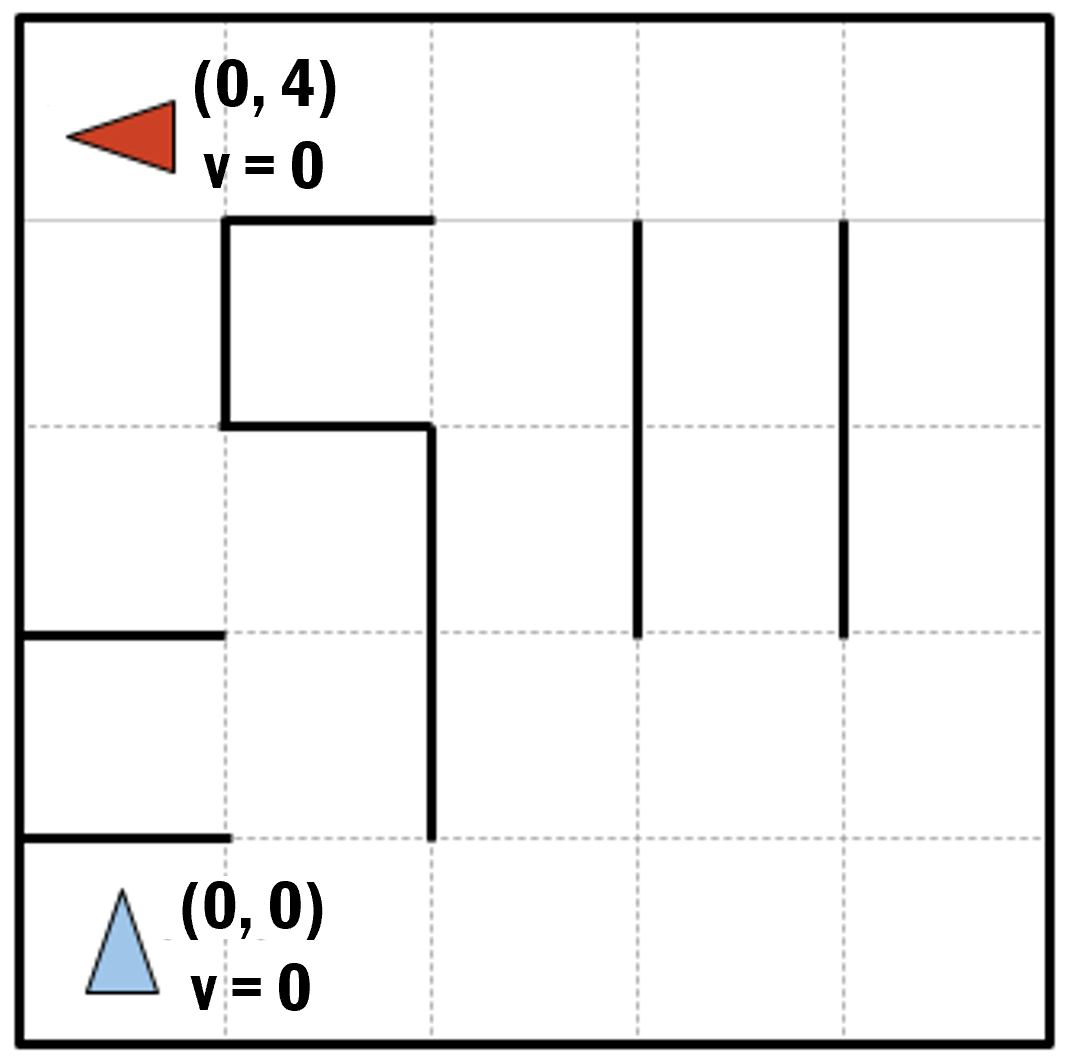
\includegraphics[scale=.33]{figures/movingagent.png} 
\end{center}

Imagine a car-like agent wishes to exit a maze like the one shown above. The agent is directional and at all times faces some direction $d \in (N, S, E, W)$. With a single action, the agent can \textit{either} move forward at an adjustable velocity $v$ or turn.

The moving actions are \textit{faster}, \textit{maintain} and \textit{slower}. For these actions, the agent then moves a number of squares equal to its \textbf{new} adjusted velocity. Let $v$ denote the agent's current velocity and let $v'$ denote the agent's new adjusted velocity.
\begin{itemize}[noitemsep,topsep=0pt]
    \item \textit{Faster}: $v'$ = $v$ + 1
    \item \textit{Slower}: $v'$ = $v$ - 1
    \item \textit{Maintain}: $v'$ = $v$
\end{itemize}

The turning actions are \textit{left} and \textit{right}, which change the agent’s direction by 90 degrees. Turning is only permitted when the velocity is zero (and leaves it at zero). 
\begin{itemize}[noitemsep,topsep=0pt]
    \item \textit{Left}: change the agent’s direction by 90 degrees counterclockwise
    \item \textit{Right}: change the agent’s direction by 90 degrees clockwise
\end{itemize}

For example, if the agent is currently on (0, 0) facing north with velocity 0 (as pictured) and wants to get to (2, 0) facing east with velocity 0, the sequence of actions will be: \textit{right, faster, maintain, slower}.

Illegal actions include
\begin{itemize}[noitemsep,topsep=0pt]
    \item Any action that would result in a collision with a wall
    \item Any action that would reduce $v$ below 0 or above a maximum speed $V_{max}$ 
    \item Maintaining a velocity of 0
\end{itemize}

The agent’s goal is to find a plan which parks it (stationary) in the goal direction on the exit square using as few actions (time steps) as possible. Note that the cost of a path is defined by the number of actions the agent takes.

\begin{question}[2] Suppose the agent wants to take the leftmost path (i.e., the one that passes through (1,2)) from the start (0,0) facing north to the goal (0,4) facing west. Write down the sequence of actions for it to take.

\solutionspace{2cm}{15cm}{Actions:}{\Onea}

\end{question}

\newpage

\begin{question}[2]
If the grid is M by N, what is the size of the state space? You should assume that all configurations are reachable from the start state.

\solutionspace{2cm}{10cm}{State Space Size:}{\Oneb}

\end{question}

\begin{question}[4] 
What is the maximum branching factor of this problem?
Draw an example state (x, y, orientation, velocity, grid/walls) that has this branching factor, and list the set of available actions. For example, in the above picture, if the agent was in (0, 0) facing North with a velocity of 0, the branching factor would be 2. The agent could either turn left or right.

You may assume that illegal actions are simply not returned by the problem model and therefore not counted in the branching factor. You do not necessarily have to use the example grid above. Make sure to label your drawing.

\solutionspace{1.5cm}{10cm}{Maximum Branching Factor:}{\Onecmax}

\solutionspace{5cm}{15cm}{Maximum Branching Example State and Available Actions:}{\Onecmaxexample}

\end{question}
 
\begin{question}[4]
Is the Manhattan distance from the agent’s location to the exit’s location admissible?

If not, draw an example state (x, y, orientation, velocity, grid/walls) where this heuristic overestimates at that state, and specify: 1) the heuristic value at that state and 2) the actual cost from that state to the goal.

You may assume that illegal actions are simply not returned by the problem model. You do not necessarily have to use the example grid above. Make sure to label your drawing, including the goal state.

\hspace{5mm}
\solution{\emptycircle}{\OnedYes} Yes
\hspace{5mm}
\solution{\emptycircle}{\OnedNo} No

\solutionspace{6cm}{15cm}{Example State, Heuristic Value, Actual Cost: }{\Onedreason}

\end{question}

\newpage
 
\begin{question}[4]
Is the following heuristic admissible? \textit{Manhattan distance / $V_{max}$}.

If not, draw an example state (x, y, orientation, velocity, grid/walls) where this heuristic overestimates at that state, and specify: 1) the heuristic value at that state and 2) the actual cost from that state to the goal.

You may assume that illegal actions are simply not returned by the problem model. You do not necessarily have to use the example grid above. Make sure to label your drawing, including the goal state.

\hspace{5mm}
\solution{\emptycircle}{\OneeYes} Yes
\hspace{5mm}
\solution{\emptycircle}{\OneeNo} No

\solutionspace{6cm}{15cm}{Example State, Heuristic Value, Actual Cost:}{\Oneereason }
\end{question}

\begin{question}[2]
If we used an inadmissible heuristic in A* search, could it change the completeness of the search? 

\hspace{5mm}
\solution{\emptycircle}{\OnefYes} Yes
\hspace{5mm}
\solution{\emptycircle}{\OnefNo} No

\solution{}{\OneFReason}
\end{question}

\begin{question}[2]
If we used an inadmissible heuristic in A* search, could it change the optimality of the search? 

\hspace{5mm}
\solution{\emptycircle}{\OnegYes} Yes
\hspace{5mm}
\solution{\emptycircle}{\OnegNo} No

\solution{}{\OneGReason}
\end{question}

\begin{question}[2]
Give a general advantage that an inadmissible heuristic might have over an admissible one.

\solutionspace{3.5cm}{15cm}{Answer:}{\Oneh}
\end{question}

\end{problem}


\newpage
\begin{problem}{Search Nodes}

Consider the tree search (i.e. no explored set) of an arbitrary search problem with max branching factor $b$. Each search node $n$ has a backward (cumulative) cost of $g(n)$, an admissible heuristic of $h(n)$, and a depth of $d(n)$. Let $n_c$ be a minimum-cost goal node, and let $n_s$ be a shallowest goal node.

For each of the following, give an expression that characterizes the set of nodes that are explored before the search terminates.
For instance, if we asked for the set of nodes with positive heuristic value, you could say: for all $n$, such that $h(n) \geq 0$. Don't worry about ties (so you won’t need to worry about $>$ versus $\geq$). If there are no nodes for which the expression is true, you must write ``none.''

\begin{question}[5]
Give an inequality in terms of the functions defined above to describe the nodes $n$ that are explored in a breadth-first search before terminating.

\solutionspace{2cm}{15cm}{Inequality: All $n$, such that:}{\Twoa}
  
\end{question}

\begin{question}[5]
Give an inequality in terms of the functions defined above to describe the nodes $n$ that are explored in a uniform cost search before terminating.

\solutionspace{2cm}{15cm}{Inequality: All $n$, such that:}{\Twob}
  
\end{question}

\begin{question}[5]
Now for this question, assume the heuristic is consistent. Give an inequality in terms of the functions defined above to describe the nodes $n$ that are explored in an A* before terminating.

\solutionspace{2cm}{15cm}{Inequality: All $n$, such that:}{\Twoc}
  
\end{question}


\end{problem}
\newpage
\begin{problem}{Searching a Graph}

\begin{table}[h]
\centering
\begin{minipage}{0.45\linewidth}
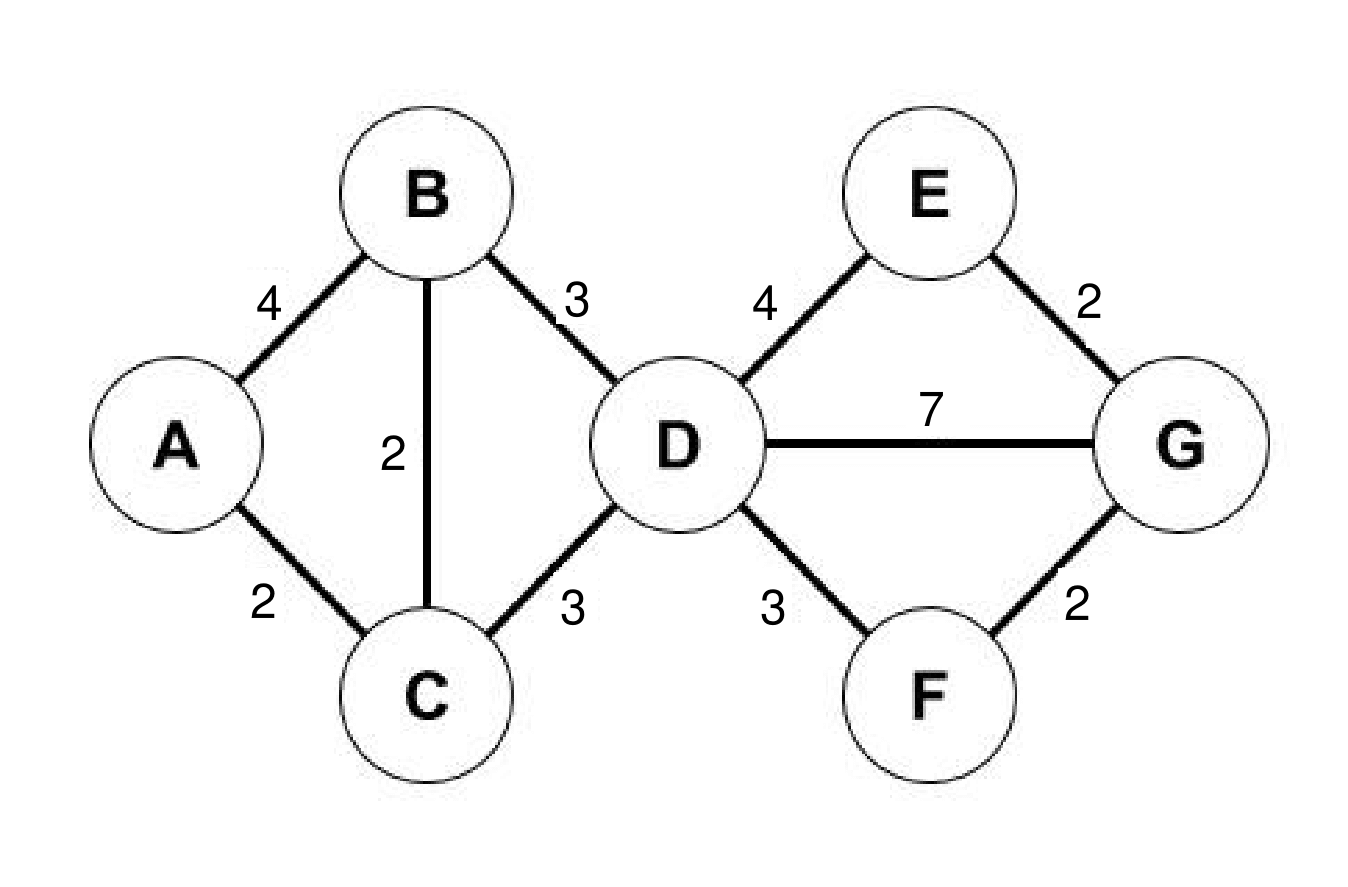
\includegraphics[scale=.5]{figures/graph2.png} 
\end{minipage}
\hspace{0.5cm}
\begin{minipage}{0.45\linewidth}
\begin{tabular}{|l|l|l|}
\hline
Node & $h_1$ & $h_2$\\
\hline
A &14 &9\\
B &10 &6\\
C &11 &7\\
D &6 &4\\
E &4 &2\\
F &5 &1.5\\
G &0 &0\\
\hline
\end{tabular}
\end{minipage}
\end{table}

Consider the state space graph shown above. A is the start state and G is the goal state. The costs for each edge are shown on the graph. Each edge can be traversed in both directions. Please refer to the search algorithms \textbf{exactly as presented on the lecture slides} as the ordering of the actions matters.

\begin{question}[15]
For each of the following \textbf{graph search} strategies, mark with an X which (if any) of the listed paths it could return. Note that for some search strategies the specific path returned might depend on tie-breaking behavior. In any such cases, make sure to mark \textbf{all} paths that could be returned under some tie-breaking scheme.


\begin{table}[h]
\begin{center}
\begin{tabular}{|l|l|l|l|}
\hline
Algorithm & A-B-D-G & A-C-D-G & A-C-D-F-G\\
\hline
UCS & \begin{minipage}{3cm}~\\(i)\quad\solution{}{\Threeai}~\\~\\\end{minipage} &
\begin{minipage}{3cm}~\\(ii)\quad\solution{}{\Threeaii}~\\~\\\end{minipage} & 
\begin{minipage}{3cm}~\\(iii)\quad\solution{}{\Threeaiii}~\\~\\\end{minipage}\\
\hline
Greedy with heuristic $h_1$ & \begin{minipage}{3cm}~\\(iv)\quad\solution{}{\Threeaiv}~\\~\\\end{minipage} &
\begin{minipage}{3cm}~\\(v)\quad\solution{}{\Threeav}~\\~\\\end{minipage} & 
\begin{minipage}{3cm}~\\(vi)\quad\solution{}{\Threeavi}~\\~\\\end{minipage}\\
\hline
Greedy with heuristic $h_2$ & \begin{minipage}{3cm}~\\(vii)\quad\solution{}{\Threeavii}~\\~\\\end{minipage} &
\begin{minipage}{3cm}~\\(viii)\quad\solution{}{\Threeaviii}~\\~\\\end{minipage} & 
\begin{minipage}{3cm}~\\(ix)\quad\solution{}{\Threeaix}~\\~\\\end{minipage}\\

\hline
A* with heuristic $h_1$ & \begin{minipage}{3cm}~\\(x)\quad\solution{}{\Threeax}~\\~\\\end{minipage} &
\begin{minipage}{3cm}~\\(xi)\quad\solution{}{\Threeaxi}~\\~\\\end{minipage} & 
\begin{minipage}{3cm}~\\(xii)\quad\solution{}{\Threeaxii}~\\~\\\end{minipage}\\
\hline
A* with heuristic $h_2$ & \begin{minipage}{3cm}~\\(xiii)\quad\solution{}{\Threeaxiii}~\\~\\\end{minipage} &
\begin{minipage}{3cm}~\\(xiv)\quad\solution{}{\Threeaxiv}~\\~\\\end{minipage} & 
\begin{minipage}{3cm}~\\(xv)\quad\solution{}{\Threeaxv}~\\~\\\end{minipage}\\
\hline
\end{tabular}
\end{center}
\end{table}
  
\end{question}

\begin{question}[1]
What is the cost of the optimal path for uniform cost search from A to G?

\solutionspace{1.2cm}{7.5cm}{Answer:}{ \Threeb}

\end{question}

\begin{question}[4]
Is $h_1$ admissible? Is it consistent?

Admissible: \hspace{5mm}
\solution{\emptycircle}{\ThreeCAdmissibleYes} Yes
\hspace{5mm}
\solution{\emptycircle}{\ThreeCAdmissibleNo} No

\solution{}{\ThreeCAdmissibleReason}

Consistent: \hspace{5mm}
\solution{\emptycircle}{\ThreeCConsistentYes} Yes
\hspace{5mm}
\solution{\emptycircle}{\ThreeCConsistentNo} No

\solution{}{\ThreeCConsistentReason}

\end{question}

\begin{question}[4]
Is $h_2$ admissible? Is it consistent?

Admissible: \hspace{5mm}
\solution{\emptycircle}{\ThreeDAdmissibleYes} Yes
\hspace{5mm}
\solution{\emptycircle}{\ThreeDAdmissibleNo} No

\solution{}{\ThreeDAdmissibleReason}

Consistent: \hspace{5mm}
\solution{\emptycircle}{\ThreeDConsistentYes} Yes
\hspace{5mm}
\solution{\emptycircle}{\ThreeDConsistentNo} No

\solution{}{\ThreeDConsistentReason}


\end{question}





\end{problem}


\newpage
\begin{problem}{Search: Multiple Choice and Short Answer Questions}

\begin{question}[12]
Consider the following true/false questions with each question worth 2 points. For the following search problems, assume every action has a cost of at least $\epsilon$, with $\epsilon > 0$.  Assume any heuristics used are consistent. 

\vspace{2mm}
\hspace{0.5mm}
Depth-first tree-search is guaranteed to be complete. \\
\solution{\emptycircle}{\FourAATrue} \textbf{True}
\hspace{5mm}
\solution{\emptycircle}{\FourAAFalse} \textbf{False} \\
\solution{}{\FourAAReason}

\vspace{2mm}
\hspace{0.5mm}
Breadth-first tree-search is guaranteed to be complete. \\
\solution{\emptycircle}{\FourABTrue} \textbf{True}
\hspace{5mm}
\solution{\emptycircle}{\FourABFalse} \textbf{False} \\
\solution{}{\FourABReason}

\vspace{2mm}
\hspace{0.5mm}
Iterative deepening tree-search is guaranteed to be complete. \\
\solution{\emptycircle}{\FourACTrue} \textbf{True}
\hspace{5mm}
\solution{\emptycircle}{\FourACFalse} \textbf{False} \\
\solution{}{\FourACReason}

\vspace{2mm}
\hspace{0.5mm}
For all graphs without cycles, graph-search contains a larger frontier than tree-search. \\
\solution{\emptycircle}{\FourADTrue} \textbf{True}
\hspace{5mm}
\solution{\emptycircle}{\FourADFalse} \textbf{False} \\
\solution{}{\FourADReason}

\vspace{2mm}
\hspace{0.5mm}
Iterative deepening graph-search has the time complexity of BFS and the space complexity of DFS. \\
\solution{\emptycircle}{\FourAETrue} \textbf{True}
\hspace{5mm}
\solution{\emptycircle}{\FourAEFalse} \textbf{False} \\
\solution{}{\FourAEReason}

\vspace{2mm}
\hspace{0.5mm}
If $h_{1}$(s) is a consistent heuristic and $h_{2}$(s) is a consistent heuristic, then min($h_{1}$(s), $h_{2}$(s)) must be consistent. \\
\solution{\emptycircle}{\FourAFTrue} \textbf{True}
\hspace{5mm}
\solution{\emptycircle}{\FourAFFalse} \textbf{False} \\
\solution{}{\FourAFReason}
\end{question} 
\vspace{2mm}

\begin{question}[5] 
Consider the state space graph shown below. S is the start state and G is the goal state. The costs for each edge are shown on the graph. For the following table below, fill in potential heuristic values such that the heuristic is admissible but not consistent. 

\vspace{10mm}
\begin{centering} 
\hspace{10mm}
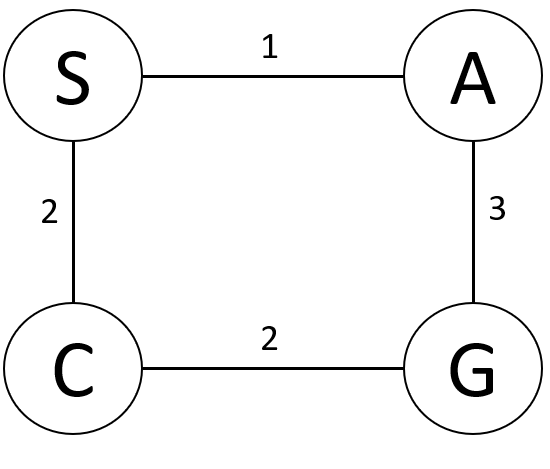
\includegraphics[scale=.6]{figures/Consistent.png} 
\hspace{32mm}{\raisebox{32mm}{
\begin{tabular}{ |p{1.8cm}|p{1.2cm}|  }
\hline
\multicolumn{2}{|c|}{\textbf{Heuristic Function}} \\
\hline
\textbf{State} & \textbf{$h(s)$}  \\
\hline
$S$ & \solution{}{\FourBS}  \\
\hline
$A$ & \solution{}{\FourBA}  \\
\hline
$C$ & \solution{}{\FourBC}   \\
\hline
$G$ &  0 \\
\hline
\end{tabular}}}
\end{centering}

\solution{}{\FourBReason}

\end{question}

\end{problem}
\newpage
\begin{problem}{Expectimax Search}
We have replaced the minimization nodes with expectation nodes (circles). Use the algorithm presented in class and the search tree to answer the following questions. Assume equal weight.

\begin{center}
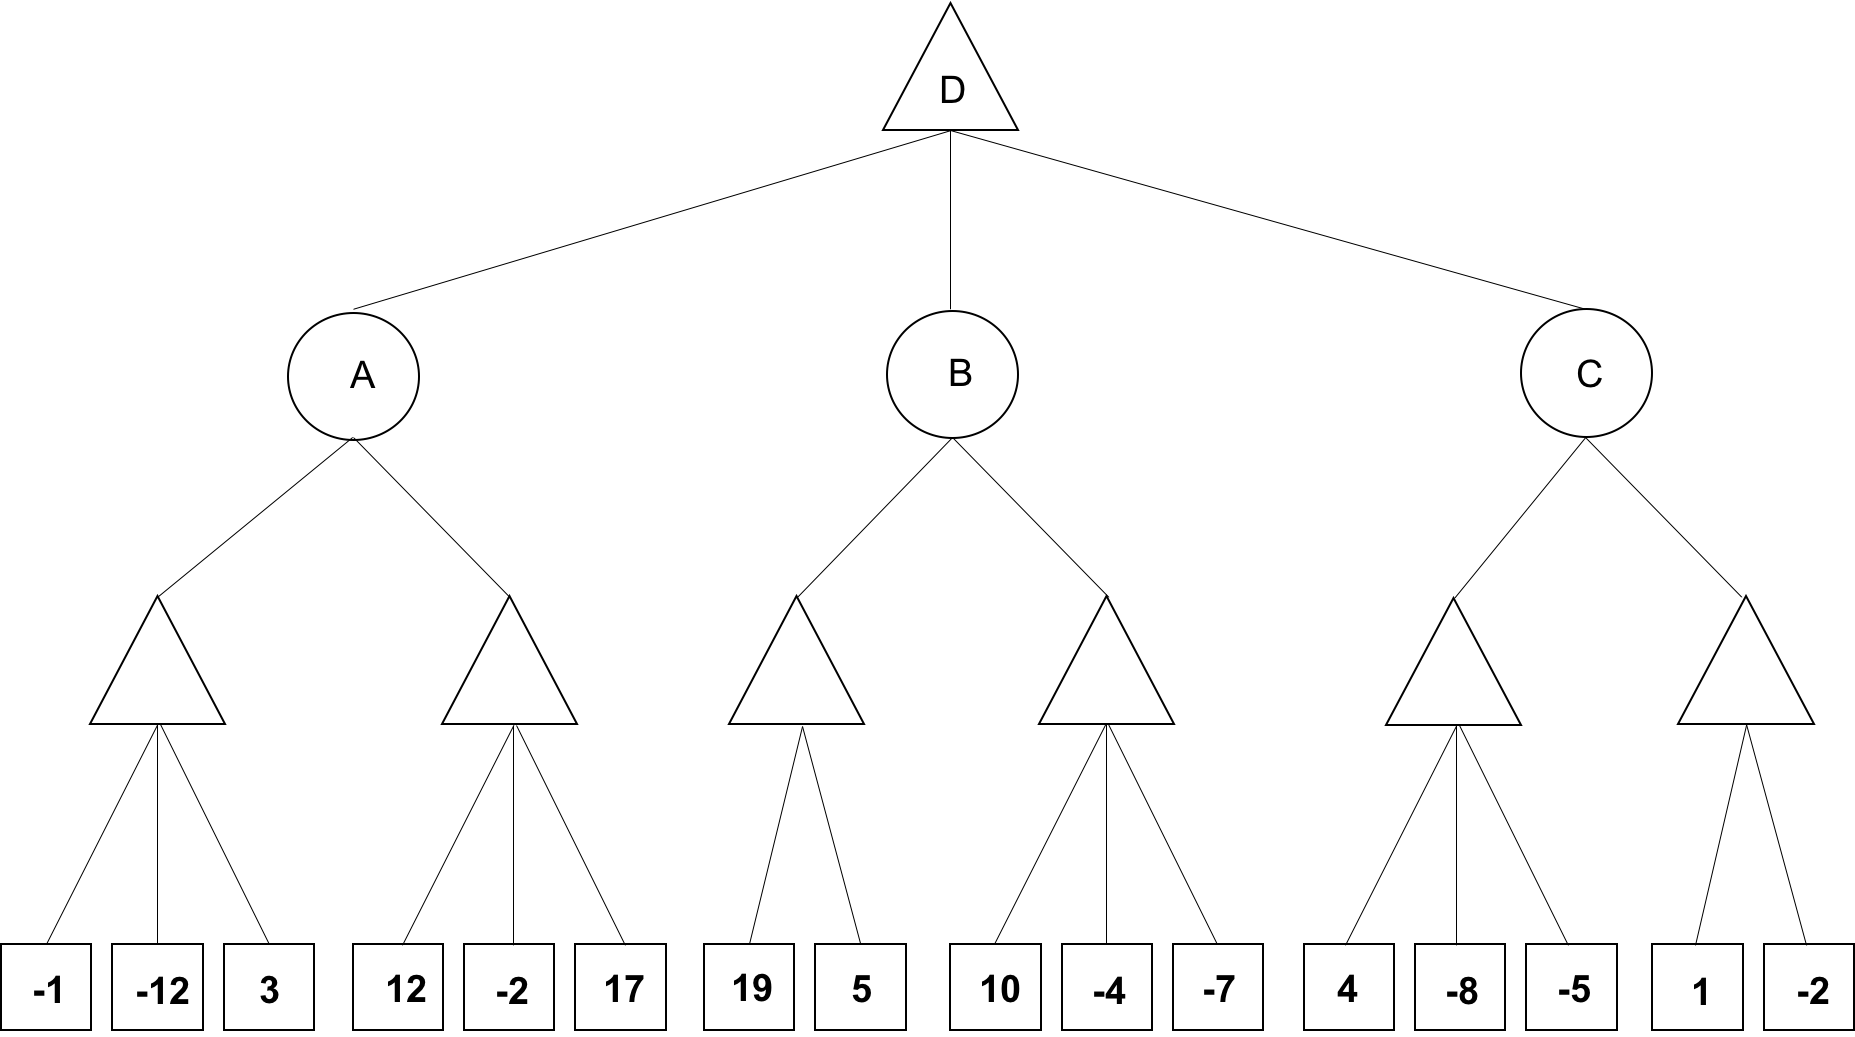
\includegraphics[width=400 pt]{figures/Expectimax-q5.png}
\end{center}

\begin{question}[2]
What is the value of node A?

\solutionspace{1.2cm}{1.5cm}{Answer:}{ \FiveA}
\end{question}

\begin{question}[2]
What is the value of node B?

\solutionspace{1.2cm}{1.5cm}{Answer:}{ \FiveB}
\end{question}

\begin{question}[2]
What is the value of node C?

\solutionspace{1.2cm}{1.5cm}{Answer:}{ \FiveC}
\end{question}

\begin{question}[2]
What is the value of node D?

\solutionspace{1.2cm}{1.5cm}{Answer:}{ \FiveD}
\end{question}

\end{problem}
\newpage
\begin{problem}{Minimax and Alpha-Beta Pruning}
Note: Triangle nodes pointing up refer to max nodes, and triangle nodes pointing down refer to min nodes.

\begin{center}
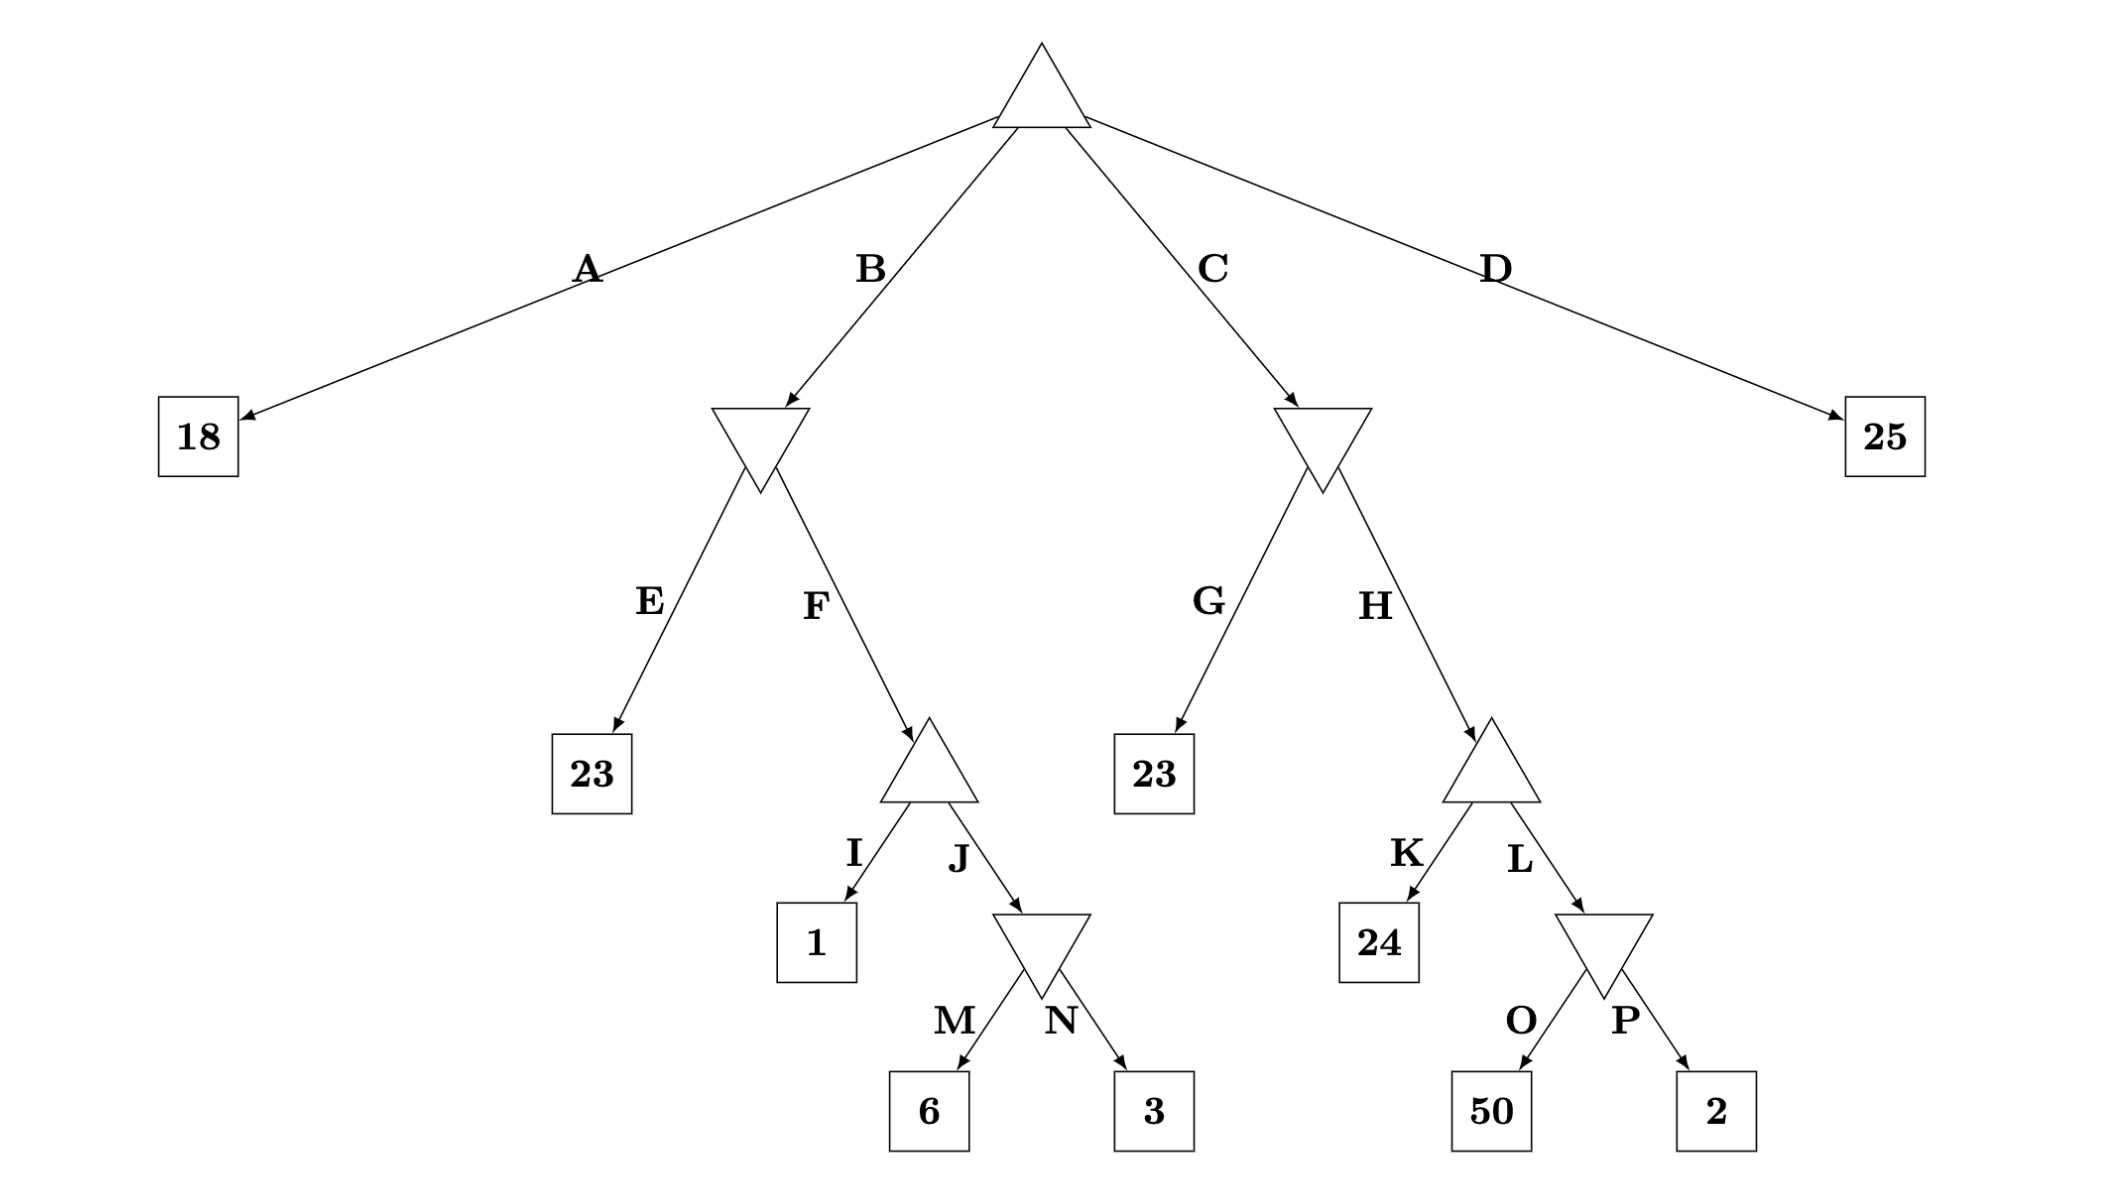
\includegraphics[width=400 pt]{figures/Minimax-and-AlphaBeta-q6.png}
\end{center}

\begin{question}[1]
What is the minimax value of the root?

\solutionspace{1.2cm}{1.5cm}{Answer:}{ \SixA}
\end{question}

\begin{question}[2]
What are the minimax value for the minimizer nodes at level 2 (assuming the root node is at level 1)?
\begin{subquestion}[1]

\solutionspace{1.2cm}{2cm}{Answer B:}{ \SixBi}
\end{subquestion}
\qquad
\begin{subquestion}[1]

\solutionspace{1.2cm}{2cm}{Answer C:}{ \SixBii}
\end{subquestion}
\end{question}

\begin{question}[4]
Assuming children are visited in left-to-right order, which branches (letters)  would be pruned by alpha-beta pruning?

NOTE: select the top most branch that can be pruned. For example, if branch B is pruned, then we know E and F are both pruned as well. However, in this case, only select B as your answer.

\solutionspace{1.2cm}{4cm}{Answer:}{ \SixC}

\end{question}

\begin{question}[4]
Which of the below orderings would result in the most pruning (select all that apply)? Assume all other nodes are visited in left-to-right order, except for children of the root. For example, if you believe left-to-right order would result in the most pruning, you should select A,B,C,D.

\solution{\emptysquare}{\SixDi} A,B,C,D
\qquad
\solution{\emptysquare}{\SixDii} C,D,A,B
\qquad
\solution{\emptysquare}{\SixDiii} D,A,B,C
\qquad
\solution{\emptysquare}{\SixDiv} D,A,C,B
\qquad
\solution{\emptysquare}{\SixDv} B,D,A,C

\end{question}
\end{problem}
\newpage
\begin{problem}{Ethics}

\begin{question}[3]
Please review this article discussed in recitation: \textit{This Navigation App Keeps You Out of High-crime Areas in Real Time},\\ \url{https://www.androidauthority.com/redzone-navigation-app-avoids-high-crime-areas-686894/}.

\begin{subquestion}[1]
Let's assume this navigation app uses A* search with an admissible and consistent heuristic to find and return paths.
Suppose you are working on this app, and your boss proposes a new heuristic.
There is some crime rate metric that ranges from 0 to 5, where 5 is high crime. 
Your boss proposes that you add this crime rate metric to the application's current heuristic, such that \textbf{the heuristic is still admissible and consistent.}

%Describe the impact this will this have on the path that is returned. Give your answer in one sentence.[
Will the path \textbf{necessarily} change with the new heuristic? If so, will the new path be optimal? If not, under what conditions would the path change?
 
\solutionspace{2cm}{15cm}{Answer:}{\SevenAi}
\end{subquestion}

\begin{subquestion}[1]
If for some reason you choose not to adjust the heuristic, what is one way your implementation could return paths that avoid high crime areas? Give your answer in one sentence.


\solutionspace{2.5cm}{15cm}{Answer:}{\SevenAii}
\end{subquestion}

\begin{subquestion}[1]
In what ways could people living in high crime neighborhoods be impacted by changes in navigation algorithms? Please provide 2-3 sentences.

\solutionspace{3cm}{15cm}{Answer:}{\SevenAiii}
\end{subquestion}

\end{question}

\end{problem}
\end{document}
